% !TeX spellcheck = es
\documentclass{report}
\usepackage[utf8]{inputenc}

% Títulos automáticos en español
\usepackage[spanish]{babel}

% Soporte para buenas urls e hipervínculos entre secciones
\usepackage{hyperref}

% Citas y referencias en formato APA
% Si quiere las citas y referencias en IEEE comente esta línea
\usepackage{apacite}

% Imágenes y figuras
\usepackage{graphicx}

% Código fuente con números de línea
\usepackage{listings}
% Puede cambiar el lenguaje de código fuente
% https://www.overleaf.com/learn/latex/code_listing#Supported_languages
\usepackage{multirow}


\lstset{
    language=C,
    basicstyle=\footnotesize,
    numbers=left,
    stepnumber=1,
    showstringspaces=false,
    tabsize=1,
    breaklines=true,
    breakatwhitespace=false,
}


\def \unidad{Escuela de Ingeniería en Computación}
\def \programa{Ingeniería en Computación}
\def \curso{IC6600 - Principios de Sistemas Operativos}
\def \titulo{Proyecto 2}
\def \subtitulo {Simulación de Algoritmos de Paginación}
\def \autores{
    Gerald Calderón\\
    gecalderon@estudiantec.cr\\
    2023125197\\
    
    \vspace{0.5cm}
    
    Óscar Obando\\
    osobando@estudiantec.cr\\
    2023091684
    
    \vspace{0.5cm}
    
    Samuel Zúñiga\\
    sazuniga@estudiantec.cr	\\
    2023029693
}
\def \fecha{Octubre 2025}
\def \lugar{
    San José, 
    Costa Rica
}

% Inicia el documento 
\begin{document}

% Inserta la portada del documento
\begin{titlepage}
    \begin{center}
        \vspace*{1cm}
        
        
\includegraphics[width=0.8\linewidth]{figuras/logo_tec.jpg}\\
        \LARGE
        \unidad\\
        \programa\\
        \curso
        
        \vspace{1cm}
        
        \Huge
        \textbf{\titulo}
            
        \vspace{0.5cm}
        \LARGE
        \subtitulo
            
        \vspace{1.5cm}
        
        \large    
        \autores
            
        \vfill
        
        \lugar\\
        \fecha
        
    \end{center}
\end{titlepage}

\tableofcontents

\chapter{Introducción}\label{intro}
Introduccion perrona

\chapter{Detalles de la implementación}
\section {Algoritmos de Paginación}
En esta sección se explican los algoritmos de paginación implementados en la simulación. 
Antes de iniciar con la explicación de cada uno, es importante recalcar que internamente la memoria es representada por un array de enteros. 
Dichos enteros representan el ID de cada página. 
Por esta estructura, cada algoritmo hace su funcionamiento normal y retorna el índice de la página que debe ser reemplazada.
Dentro de la MMU se maneja qué ocurre si la página ya está en memoria o si la memoria tiene espacio, por lo que la única responsabilidad de cada algoritmo es decidir cuál página reemplazar.

\subsection{Óptimo}
[PONER REFERENCIOA]
El algoritmo óptimo de paginación es aquel que tiene la capacidad de ver el futuro, es decir, sabe cuales páginas serán utilizadas durante toda la ejecución de la máquina para poder decider a cual mandaar a memoria virtual. Su funcionamiento consiste en buscar dentro de las páginas cargadas en memoria real aquella que nunca se va a volver a utilizar o la que se va a utilizar más tarde para reemplazarla por la que se requiera cargar en dicho momento. \\


Para su implementación al leer el archivo de instrucciones a utilizar se llama a la función ``parse\_for\_optimal" (ver figura \ref{fig:parse_optimal})que detecta cada aparición de ``use" o ``new" para registrar las páginas en una lista que contendrá el id de las páginas que son utilizadas en dichas instrucciones. Una vez se lee todo el archivo dicha lista de páginas es pasada al constructor de la MMU concreta que contiene el algoritmo óptimo como implementación de la función ``paging" (ver figura \ref{fig:optimal}).

\begin{figure}[h]
	\centering
	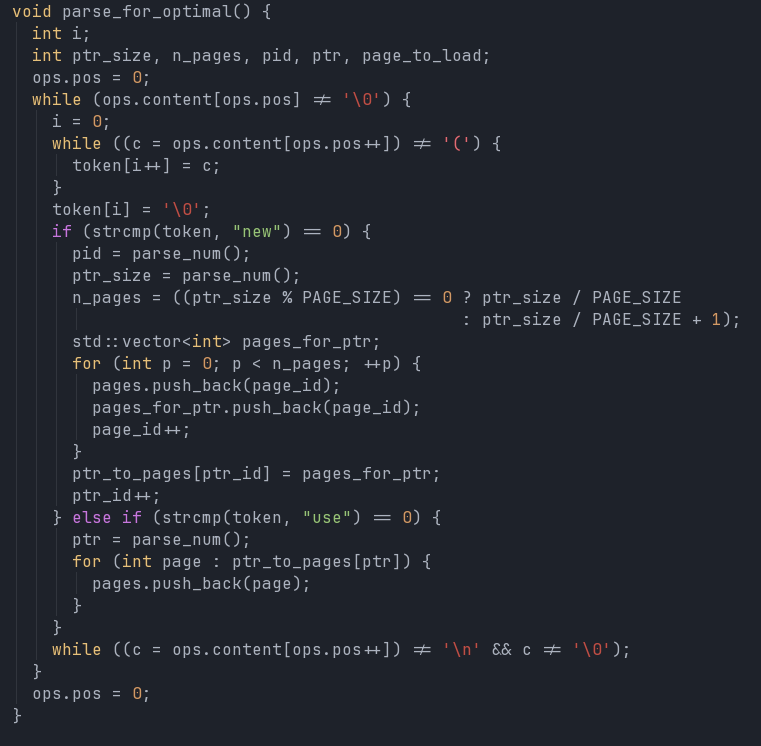
\includegraphics[width=0.8\linewidth]{figuras/parse_optimal.png}
    \caption{Ilustración de la función que obtiene todas las páginas que se usarán}
	\label{fig:parse_optimal}
\end{figure}

\begin{figure}[h]
	\centering
	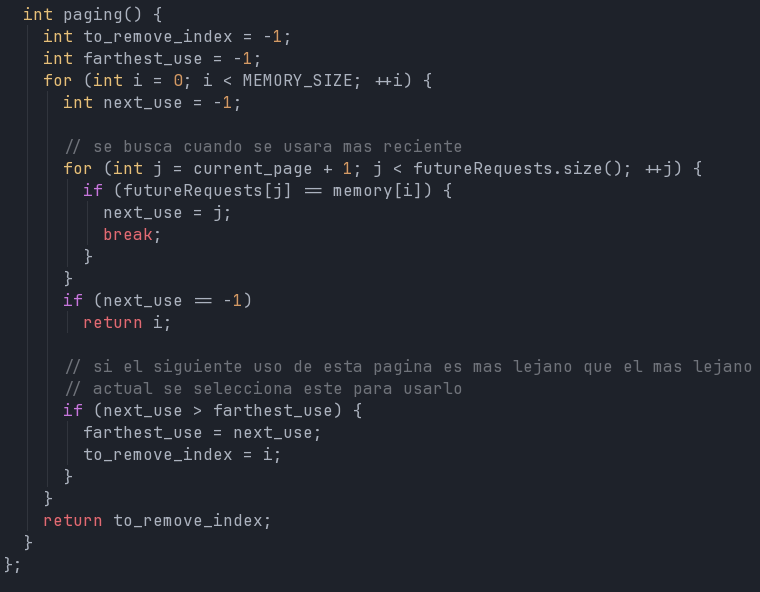
\includegraphics[width=0.8\linewidth]{figuras/optimal.png}
	\caption{Ilustración de el algoritmo óptimo}
	\label{fig:optimal}
\end{figure}


\subsection{FIFO y Second Chance}
\subsubsection{FIFO}
[PONER REFERENCIOA]
El algoritmo FIFO es (junto a Random) el algoritmo más simple impementado para manejar paginación en el programa.
Este algoritmo por sus siglas significa "First in - First Out``, como su nombre lo indica, este consiste en sacar la página que lleva más tiempo en memoria para dar espacio a las demás. \\


Para implementar esto, se decidió utilizar dos variables "to\_remove\_index``(el índice de la página que se va a remover) y "time\_loaded``(el tiempo que la página lleva cargada). 
Por defecto ambas se setean en -1, este valor es reescrito en el momento que se ejecuta la lógica del algoritmo.
Dentro de un for loop se revisan todas las páginas dentro de memoria, si la cantidad de tiempo que esa página es mayor a la cantidad guardada en "time\_loaded`` se actualiza el índice y dicha variable.
De esta forma, una vez termina el for loop, se tiene el índice de la página que lleva más tiempo cargada, una vez hecho esto simplemente se retorna este índice.
Este comportamiento se puede ver en el código mostrado en la Figura \ref{fig:fifo}.

\begin{figure}[h]
	\centering
	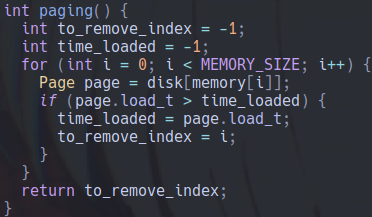
\includegraphics[width=0.8\linewidth]{figuras/fifo.png}
	\caption{Ilustración de el algoritmo FIFO}
	\label{fig:fifo}
\end{figure}

\subsubsection{Second Chance}
[PONER REFERENCIOA]

\subsection{LRU y MRU}
\subsubsection{LRU}
[PONER REFERENCIOA]
\subsubsection{MRU}
[PONER REFERENCIOA]

\subsection{Random}
[PONER REFERENCIOA]


\chapter{Instrucciones para el uso del programa}
\section{Cómo instalar el programa}
\begin{enumerate}
  \item Descargue el código fuente del programa. Puede hacerlo de las dos siguientes formas:
    \begin{itemize}
      \item Dirigirse al repositorio de GitHugitb mediante su navegador a través del siguiente link: \url{https://github.com/Andres2950/PSO\_PagingSimulator.git}
      \item Instalarlo directamente con el comando \\
    \texttt{wget \url{https://github.com/Andres2950/PSO\_PagingSimulator/archive/refs/heads/main.zip}}
    \end{itemize}
  \item Descomprima el archivo .zip descargado utilizando el comando \texttt{unzip}.
  \item Al extraer el archivo podrá observar la estructura de organización similar a la figura \ref{fig:estructura}.
\item Ejecute el archivo \texttt{install.sh}, asegúrese de qué tenga permisos de ejecución, puede utilizar el comando \texttt{chmod +x install.sh} en caso de que no los posea y luego ejecute de la siguiente forma \texttt{./install.sh}. \\
  Este archivo se hará cargo de la instalación del compilador \textit{g++} necesario para compilar el código fuente. Además hará la instalación del paquete \textit{cmake} para la ejecución del archivo ``CMakeLists.txt", dicho archivo posee las instrucciones de compilación de \textit{SDL} para resolver todas las dependencias. 
\item Note que la instalación de dichos paquetes requiere permisos de usuarios root, al ejecutar el archivo \texttt{install.sh} este se volverá a ejecutar con dichos permisos, para esto solicitará la contraseña del usuario root para tener dichos permisos de ejecución (la contraseña es totalmente invisible para el programa) y así poder descargar los paquetes.
\item La compilación de los archivos se realiza sin permisos root.
%\item Además, el \texttt{install.sh} hará una copia de los binarios \texttt{huff} y \%texttt{dehuff} en el directorio \textit{/usr/bin} de la máquina para poner ser %accedidos desde cualquier lugar y utilizado en múltiples directorios sin necesidad %de mover los archivos a comprimir o descomprimir a una carpeta en particular.

\end{enumerate}


\section{Cómo utilizar el programa}
Una vez terminado el procedimiento de instalar el programa puede utilizar el comando \texttt{./build/app/app} en la carpeta del proyecto descargada para ejecutar el programa de simulación.



\chapter{Conclusiones}


% Estilo de bibliografía APA
% Si quiere usar el estilo IEEE comente esta línea
\bibliographystyle{apacite}

% Descomente esta línea para usar el estilo de bibliografía IEEE
%\bibliographystyle{ieeetr}
\bibliography{referencias}

\end{document}
